\documentclass{standalone}
\author{Quinten Bruynseraede}
\usepackage{tikz}
\usetikzlibrary{shapes}
\title{Tikz grafen}
\begin{document}\pagestyle{empty}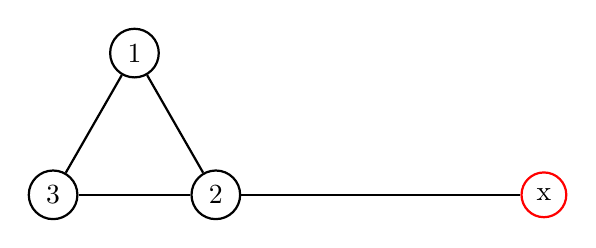
\begin{tikzpicture}\node[shape=circle,draw=black,align=center,line width=0.8pt] (0) at (2.6,12.166666666666666) {1};
\node[shape=circle,draw=black,align=center,line width=0.8pt] (1) at (1.5666666666666667,10.366666666666667) {3};
\node[shape=circle,draw=black,align=center,line width=0.8pt] (2) at (3.6333333333333333,10.366666666666667) {2};
\node[shape=circle,draw=red,align=center,line width=0.8pt] (3) at (7.8,10.366666666666667) {x};

\path [-,draw=black,line width=0.8pt] (1) edge node {} (2);
\path [-,draw=black,line width=0.8pt] (2) edge node {} (0);
\path [-,draw=black,line width=0.8pt] (0) edge node {} (1);
\path [-,draw=black,line width=0.8pt] (2) edge node {} (3);
\end{tikzpicture}
\end{document}